\chapter{Clustering}
Il \textbf{clustering} è un approccio non supervisionato. Come se stessimo
lavorando ``ad occhio'' si potrebbero avere vari criteri per effettuare il
raggruppamento delle istanze, in mancanza di label. Il criterio di scelta è
praticamente arbitrario e il termine ``classificare'' diventa più un
``raggruppare''. Il sistema è quindi flessibile nel decidere i criteri (che non
può essere scelto in base alle label) sfruttando concetti come la distribuzione
dei dati. I risultati ottenuti da un apprendimento
non supervisionato potrebbero ``sorprendere'' in quanto potrebbero essere
imprevedibili a priori. In ogni caso l'incertezza del clustering non è la sola,
in quanto anche un sistema supervisionato potrebbe comunque lasciare spazio ad
incertezza sulle ipotesi (non riuscendo magari ad avere tutte le label possibili
per l'insieme dei casi).\\ 
Possiamo pensare di rappresentare nello spazio (con dimensione pari al numero di
attributi delle istanze) le varie istanze per poi cercare di capire come
etichettare le varie istanze la cui etichetta non è nota. Si procede quindi
\textbf{raggruppando per distanza} (se è vicina a istanze con una certa
etichetta nota uguale anche istanza di cui cerchiamo l'etichetta avrà
quell'etichetta), usando la \textit{distanza di Hamming} o la \textit{distanza
  Euclidea}, ma prima di parlarne introduciamo meglio tutto il discorso. \\
La ``decisione forte'' è raggruppare e quindi scegliere in base alla distanza,
definendo prima la distanza stessa, misurando poi il risultato secondo un certo
criterio di misura (sempre basato sulla distanza).\\
Avendo una classificazione non supervisionata si ha una scarsa conoscenza a
priori dei dati da analizzare, puntando quindi all'estrazione automatica delle
classi mentre in quella supervisionata si partiva da classi etichettate, avendo
magari speso costo computazionale per ottenerle, e e da una struttura
classificatoria conosciuta (avendo un set d'ipotesi possibili). I sistemi non
supervisionati tornano comodo quando la distribuzione dei valori degli attributi
è informazione sufficiente per separare le istanze in più classi, si hanno
quindi domini dove questo fattore è determinante. Con l'apprendimento non
supervisionato quindi la non conoscenza a priori è anche un vantaggio (magari le
etichette che uso nel supervisionato potrebbero essere errate), insieme
alla riduzione dell'errore umano. Un altro pro è che tutte le classi con
caratteristiche uniche vengono identificati e quindi i metodi di apprendimento
non supervisionato sono efficaci con elementi di tipo numerico, che diventano
coordinate in uno spazio, e con elementi dotati di ordinamento intrinseco, per
il calcolo delle distanze. Di contro le classi ottenute non per forza hanno un
significato. Inoltre l'utente ha poco controllo sulla procedura e sui risultati
e tali metodi sono meno efficaci con elementi ordinati in modo arbitrario o
parziale. \\
Si cerca quindi di separare un insieme di elementi in sottoinsiemi con elementi
accomunati da caratteristiche comuni, in base a uno o più attributi con la
scelta dell'attributo viene fatta dall'algoritmo di apprendimento. Tra i campi
d'intersse si hanno:
\begin{itemize}
  \item data mining
  \item pattern recognition
  \item image analysis 
  \item bioinformatica 
  \item ricerche di mercato
  \item pianificazione urbana 
  \item sismologia 
  \item astronomia
\end{itemize}
Ogni elemento da classificare viene specificato da un vettore caratteristico e
si ha una misura di similarità tra elementi. Si hanno quindi due criteri da 
rispettare:
\begin{itemize}
  \item \textbf{omogeneità} quando elementi dello stesso cluster hanno alto
  livello di similarità, quindi dentro il cluster
  \item \textbf{separazione} quando elementi di cluster diversi hanno basso
  livello di similarità, quindi tra cluster
\end{itemize}
\begin{definizione}
  Dato $N=\{e_1,\ldots, e_n\}$ un insieme di $n$ elementi e sia
  $C=\{C_1,\ldots, C_k\}$ una partizione di $N$ in sottoinsiemi. Ogni $C_i$ è
  detto \textbf{cluster} e $C$ è detto \textbf{clustering} di $N$.
\end{definizione}
\begin{definizione}
  Dati due elementi di $N$ essi sono \textbf{mates} rispetto a $C$ se
  appartenenti allo stesso cluster $C_i$
\end{definizione}
Un elemento può essere rappresentato da un vettore di numeri reali, ciascuno dei
quali misura una specifica caratteristica (feature).\\
\begin{definizione}
  Definiamo la \textbf{misura di similarità} tramite la \textbf{distanza tra
    vettori}. Si hanno tre distanze:
  \begin{itemize}
    \item la \textbf{distanza euclidea} (che è la solita distanza ottenuta dal
    definizione di Pitagora, è semplicemente la lunghezza del segmento che collega
    due punti nello spazio):
    \[d(\vec{x},\vec{y})=\sqrt{\sum_i (x_i-y_i)^2}\]
    è invariante rispetto alle  traslazioni e rotazioni degli assi
    \item la \textbf{distanza di Manhattan} (misuro gli spostamenti, che hanno
    peso 1, tra due punti in termini di somma ti tali spostamenti che formano
    una linea spezzata):
    \[d(\vec{x},\vec{y})=\sum_i (x_i-y_i)\]
    Non è invariante rispetto a traslazioni o rotazioni degli assi e pone meno
    enfasi sulle variabili con distanze maggiori, non elevando al quadrato le
    differenze
    
    \item la \textbf{distanza di Minkowski} (dando un peso diverso rispetto alla
    distanza euclidea):
    \[d(\vec{x},\vec{y})=\sqrt[k]{\sum_i (x_i-y_i)^k}\]
    In altri termini questa è la forma generica, infatti al variare di $k$ si
    hanno le varie distanze:
    \begin{itemize}
      \item con $k=1$ ottengo la distanza di Manhattan
      \item con $k=2$ ottengo la distanza euclidea
      \item con $k=\infty$ ottengo la distanza di Lagrange-\v{C}eby\v{s}\"{e}v
    \end{itemize}
    Useremo soprattutto il caso euclideo.
  \end{itemize}
\end{definizione}
In generale si hanno varie tipologie di clustering, come da figura \ref{fig:clu}
in base all'approccio di studio delle istanze o di studio dei confini tra
cluster. Questo discorso non lo approfondiremo ma si ha:
\begin{itemize}
  \item \textbf{gerarchico} quando collocano gli elementi in input in una
  struttura gerarchica ad albero, in cui le distanze tra nodi riflettono le
  similarità degli elementi. Gli elementi sono localizzati sulle foglie
  dell’albero. Come pro si ha intuitività grazie a una struttura singola,
  coerente e globale. Si ha quindi:
  \begin{itemize}
    \item \textbf{Agglomerativi} quando bisogna scegliere la coppia di cluster da fondere
    \item \textbf{divisivi}, quando si deve determinare il cluster da dividere
  \end{itemize}
  Come algoritmi si hanno:
  \begin{itemize}
    \item Neighbor joining
    \item Metodo del centroid
  \end{itemize}
  \item \textbf{non gerarchico/partitivo} quando mirano a ripartire le $n$ unità
  della popolazione in $K$ gruppi, fornendo una sola partizione anziché una
  successione di partizioni tipica dei metodi gerarchici.\\
  Come algoritmo si ha, ad esempio, \textbf{K-means}
  definendo $K$ cluster tali per cui si abbiano punti vicini in cluster
  separati. È un algoritmo iterativo
\end{itemize}
\begin{figure}
  \centering
  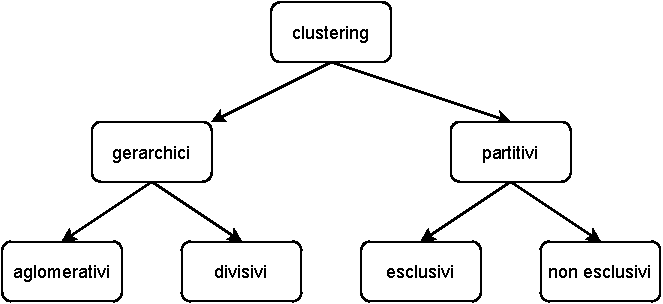
\includegraphics[scale = 1]{img/clu.pdf}
  \caption{Albero delle tipologie di clustering}
  \label{fig:clu}
\end{figure}
\section{K-Means}
\begin{definizione}
  definiamo \textbf{dendrogramma} come un albero (grafo) utilizzato per
  visualizzare la somiglianza nel processo di ``raggruppamento''.
  
\end{definizione}
Questi algoritmo è quello che vedremo per il metodo non approssimato. Si ha che
la  soluzione non è visualizzabile attraverso dendrogrammi e assume che il
numeor $K$ di cluster sia noto, puntando a minimizzare le distanze tra elementi
e i centroidi (un punto geometrico di riferimento per i cluster) dei clusters
loro assegnati.\\
L'algoritmo lavora con dati numerici in cinque step:
\begin{enumerate}
  \item si fissano a caso $K$ centroid'iniziali di altrettanti cluster
  \item per ogni elemento si calcola la distanza da ciascun centroide e lo si
  assegna al più vicino. Questo è uno step di classificazione, scegliendo il cluster
  per un elemento dato il centroide del cluster
  \item per la partizione provvisoria così ottenuta si ricalcolano i centroidi
  di ogni cluster, usando media aritmetica dei punti del cluster parziale,
  ottenendo il nuovo centroide. Si aggiustano quindi tutti i centroidi
  \item per ogni individuo si ricalcola la distanza dai centroidi e si
  effettuano gli eventuali spostamenti tra cluster dei vari elementi in base al
  fatto che si hanno nuovi centroidi
  \item si ripetono le operazioni 3 e 4 finché si raggiunge il numero massimo di
  iterazioni impostate, avendo un euristica, o non si verificano altri
  spostamenti, avendo una stabilità di risultato, avendo il risultato
  ``migliore'' 
\end{enumerate}
Si nota quindi la semplicità d'implementazione e un tempo di calcolo in :
\[O(tKn)\]
con:
\begin{itemize}
  \item $n$ cardinalità dell'insieme dei dati
  \item $K$ numero di cluster
  \item $t$ numero d'iterazioni del ciclo (avendo quindi $kt<<n$)
\end{itemize}
Di contro si ha una sensibilità rispetto alla scelta dei centroidi
iniziali, sperimentalmente si è dimostrato che brutti valori iniziali corrompano
l'intero processo. Inoltre, come detto all'inizio, non si può predire il numero
di cluster non conoscendo a priori i dati e non esiste un $K$ ottimale e non ci
sono proprietà che ce lo possano suggerire. \\
In ogni caso mappa sensatamente i vari elementi in base alle loro
caratteristiche e quindi è un approccio parecchio usato, essendo generalmente
efficacie.\\
Non sapendo a priori il numero di $K$ posso ottenere scarsi risultati magari non
avendo abbastanza centroidi. Adattarsi a un numero
``eerato'' di centroidi può portare a risultati ``sporchi''. \\
Un altro problema è dato da dati distribuiti secondo diverse ``dimensioni''
nello spazio ma l'algoritmo lavorando sui centroidi potrebbe misclassificare
questo dettaglio, non distinguendo i corretti insiemi di punti. Analogamente
succede se si hanno insiemi di punti più o meno densi, portando a
misclassicazioni. Sempre in modo analogo le proprietà di distribuzione
geometrica degli elementi comporta problemi (anche con un $K$ adeguato).

Per superare queste difficoltà si può provare ad aumentare il numero di cluster,
unendo poi, in un secondo passaggio, i vari cluster secondo certi criteri,
magari avendo una netta separazione lineare tra cluster.\\
\begin{figure}
  \centering
  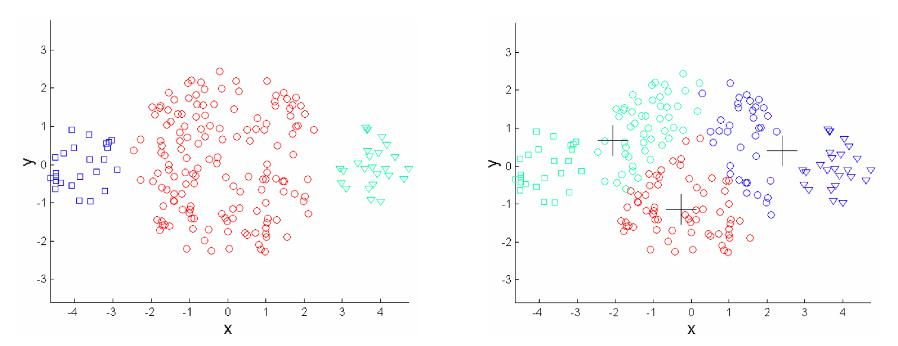
\includegraphics[scale = 0.4]{img/clu1.jpg}
  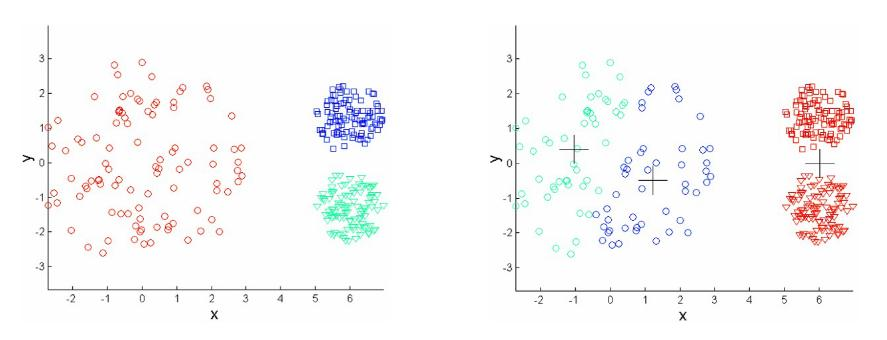
\includegraphics[scale = 0.4]{img/clu2.jpg}
  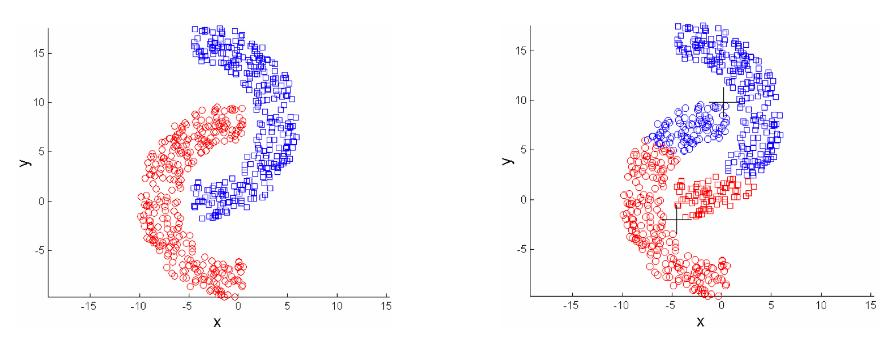
\includegraphics[scale = 0.4]{img/clu3.jpg}
  \caption{Esempi di problematiche per il clustering. A sinistra il valore
    atteso e a destra quello ottenuto. Prima si ha il problema di cluster con
    diverse dimensioni, poi con diverse densità e infine con problemi di
    proprietà geometriche.}
\end{figure}
\begin{figure}
  \centering
  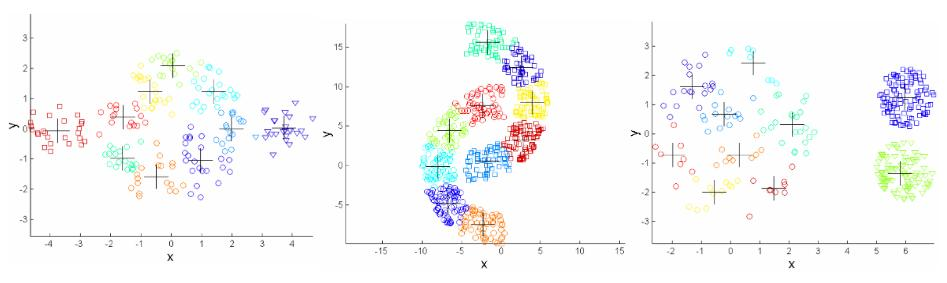
\includegraphics[scale = 0.4]{img/clusol.jpg}
  \caption{Esempi di risoluzione delle tre problematiche aggiungendo cluster.}
\end{figure}
Per misurare le prestazioni di clustering bisogna capire come classificare i
risultati. Si usa la \textbf{misura di silhouette} per capire se un clustering è
migliore di un altro. Tale misura si basa sempre sul concetto di distanza. Si
ha una tecnica di misura, supponendo che ogni cluster abbia almeno due
elementi, avendo tecniche diverse qualora si abbia cardinalità 1, avendo la
distanza tra due elementi $d(i, j)$ e due concetti:
\begin{enumerate}
  \item \textbf{distanza media ``intra-cluster''}, ovvero dentro i cluster
  \[a(i)=\frac{1}{|C_i|-1}\sum_{j\in C_i, i\neq j}d(i, j)\]
  è buono se il valore è basso
  \item \textbf{distanza media ``inter-cluster''}, ovvero tra cluster:
  \[b(i)=\min_{k\neq i}\frac{1}{|C_k|}\sum_{j\in C_k}d(i, j)\]
  è buono se il valore è alto
\end{enumerate}
ottenendo quindi la \textbf{silhouette per il punto $i$}:
\[s(i)=\frac{b(i)-a(i)}{\max{a(i), b(i)}}\]

La qualità viene quindi visualizzata da un diagramma che studia la silhouette al
variare di $K$ per ogni valore di ogni attributo (mettendo per ogni attributo in
alto i valori più studiabili).\\
La media $s(i)$ su tutti i punti di un cluster è una misura di quanto siano
strettamente raggruppati tutti i punti del cluster. Pertanto, la media s (i) su
tutti i dati dell'intero set di dati è una misura di quanto adeguatamente i dati
sono stati raggruppati. Se ci sono troppi o troppo pochi cluster, come può
accadere quando una scelta sbagliata di $k$ viene utilizzata nell'algoritmo di
clustering, alcuni dei cluster mostreranno tipicamente
linee molto più strette rispetto al resto nel diagramma di silhouette. Quindi
grafici e media di silhouette 
possono essere utilizzati per determinare il numero ``naturale'' di cluster
all'interno di un set di dati. 
\subsubsection{Esercitazione clustering e K-Means}
\begin{esercizio}
  Siano dati i seguenti 8 esempi:
  \begin{enumerate}
    \item $A1=(1, 10)$
    \item $A2=(2, 5)$
    \item $A3=(8, 4)$
    \item $A4=(5, 8)$
    \item $A5=(7, 5)$
    \item $A6=(6, 4)$
    \item $A7=(1, 2)$
    \item $A8=(4, 9)$
  \end{enumerate}
  $K=3$ e la distanza euclidea.\\
  Si supponga che all'inizio i tre centroidi (rispettivamente $seed1$, $seed2$ e
  $seed$3) siano $A1$, $A4$ e $A7$ avendo: 
  \begin{figure}[H]
    \centering
    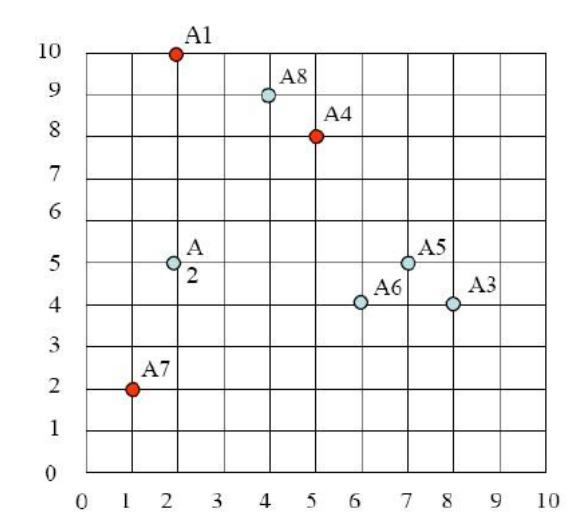
\includegraphics[scale = 0.4]{img/clue.jpg}
  \end{figure}
  \noindent
  e si esegua un'iterazione per ricalcolare i centroidi e i cluster associati.\\
  Usando la distanza euclidea procedo coi calcoli per generare i cluster,
  associando il cluster scegliendo il centroide che dista meno:
  \begin{itemize}
    \item per $A1$:
    \begin{itemize}
      \item $d(A1, seed1)=0$ essendo $A1$ il $seed1$ attuale
      \item $d(A1, seed2)=3.6$
      \item $d(A1, seed3)=8.06$
    \end{itemize}
    quindi $A1\in cluster1$
    \item per $A2$:
    \begin{itemize}
      \item $d(A2, seed1)=5$ 
      \item $d(A2, seed2)=4.24$
      \item $d(A2, seed3)=3.16$
    \end{itemize}
    quindi $A2\in cluster3$
    \item per $A3$:
    \begin{itemize}
      \item $d(A3, seed1)=6$ 
      \item $d(A3, seed2)=5$
      \item $d(A3, seed3)=7.28$
    \end{itemize}
    quindi $A3\in cluster2$
    \item per $A4$:
    \begin{itemize}
      \item $d(A4, seed1)=2.6$ 
      \item $d(A4, seed2)=0$ essendo $A4$ il $seed2$ attuale
      \item $d(A4, seed3)=7.21$
    \end{itemize}
    quindi $A4\in cluster2$
    \item per $A5$:
    \begin{itemize}
      \item $d(A5, seed1)=7.07$ 
      \item $d(A5, seed2)=3.6$
      \item $d(A5, seed3)=6.7$
    \end{itemize}
    quindi $A5\in cluster2$
    \item per $A6$:
    \begin{itemize}
      \item $d(A6, seed1)=7.21$ 
      \item $d(A6, seed2)=4.12$
      \item $d(A6, seed3)=5.38$
    \end{itemize}
    quindi $A6\in cluster2$
    \item per $A7$:
    \begin{itemize}
      \item $d(A7, seed1)=8.06$ 
      \item $d(A7, seed2)=7.21$ 
      \item $d(A7, seed3)=0$ essendo $A7$ il $seed3$ attuale
    \end{itemize}
    quindi $A7\in cluster3$
    \item per $A8$:
    \begin{itemize}
      \item $d(A8, seed1)=5$ 
      \item $d(A8, seed2)=2$
      \item $d(A8, seed3)=7.6$
    \end{itemize}
    quindi $A8\in cluster2$
  \end{itemize}
  Quindi nei nuovi cluster si ha:
  \begin{itemize}
    \item $cluster1=\{A1\}$
    \item $cluster2=\{A3, A4, A5, A6, A8\}$
    \item $cluster3=\{A2, A7\}$
  \end{itemize}
  Visualmente:
  \begin{figure}[H]
    \centering
    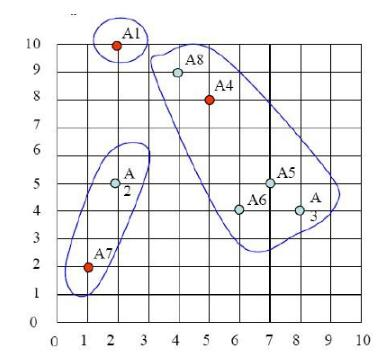
\includegraphics[scale = 0.4]{img/clue2.jpg}
  \end{figure}
  Posso fare le medie dei punti di ogni cluster per calcolare i nuovi
  centroidi: 
  \begin{itemize}
    \item $seed1New=(2, 10)$
    \item $seed2New=\left(\frac{8+5+7+6+4}{5},\frac{4+8+5+4+9}{5}\right)=(6, 6)$
    \item $seed3New=\left(\frac{2+1}{2},\frac{5+2}{2}\right)=(1.5, 3.5)$
  \end{itemize}
  Ovvero, segnando con una $x$ rossa i nuovi centroidi:
  \begin{figure}[H]
    \centering
    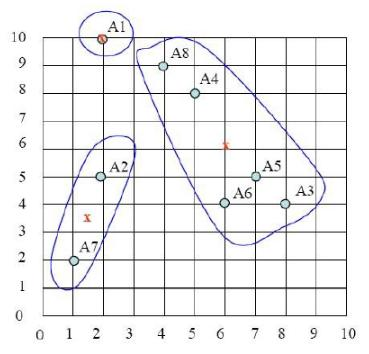
\includegraphics[scale = 0.4]{img/clue3.jpg}
  \end{figure}
  Avendo una sola epoca da calcolare mi fermo.
\end{esercizio}
\chapter{Reinforcement learning}
\textit{Brevissima introduzione a caso}.\\
Questi metodi sono usati spesso in ambienti in cui serve trainare una macchina
magari per giocare a un gioco.\\
Si inserisce una maggiore ``distanza'' tra l'errore di prestazione del sistema e
la modalità di affinamento del comportamento. In questo tipo di apprendimento
l'errore è rappresentato come premio/punizione per il comportamento, non
vedendolo più come ``distanza'' per come era intesa in concept learning, SVM,
reti etc$\ldots$.\\
Quindi, nell'esempio di un gioco, si ha un ambiente con delle regole e dei
punteggi e questi vengono usati per il training, modificando il comportamento in
base ai punti, modificando le policy del comportamento. L'algoritmo che deve
cambiare le azioni dell'\textbf{agente} in base alle indicazioni dell'ambiente è
il fulcro del reinforcement learning. La definizione di tale algoritmo è quindi
ad hoc sul sistema in analisi e avere più informazioni implica una migliore
evoluzione. La variante più grossa è capire cosa si ha sbagliato in base ai
punti ottenuti.  \\
\textbf{Non si vede altro in merito.}
\chapter{Deep learning}
\textit{Brevissima introduzione, nelle slide c'è un approfondimento. L'argomento
comunque pare non essere nel programma d'esame (il prof l'ha detto due
volte)}.\\ 
Ad oggi la fama dei sistemi di apprendimento è associata al \textbf{deep
  learning}.\\
Dalle reti neurali si passa a reti multi-layer ``complete'', con algoritmi di
discesa del gradiente, funzioni di attivazioni, strumenti di regolarizzazione,
dati (tanti) e calcoli (tanti). Si hanno quindi sia aspetti qualitativi (come
l'uso di strumenti di regolarizzazione) che quantitativi (dati e calcoli).\\
Bisogna quindi studiare algoritmi di learning anche in queste ``nuove reti'',
per esempio appunto le \textbf{deep neural net}. Potrei avere anche reti con
cicli tra le sinapsi, ricorrenze, salvataggio in memoria, studi temporali
etc$\ldots$, \textbf{convultional neural net} e \textbf{recurrent neural net}
etc$\ldots$ (per uno schema vedere figura \ref{fig:neu}). Spesso tali reti sono
usate nel riconoscimento d'immagini, soprattutto le \textit{convultional
  neural net} (anche il passaggio da immagine a feature, prima manuale, è
stato integrato nelle reti). Si ha quindi un arricchimento di quanto studiato
fin'ora.\\
\begin{figure}
  \centering
  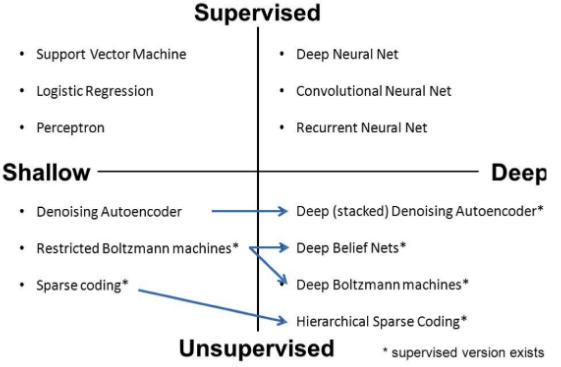
\includegraphics[scale = 0.6]{img/neu.jpg}
  \caption{Tassonometria delle reti neurali}
  \label{fig:neu}
\end{figure}
Una rete tradizionale, magari con due livelli (uno d'input e uno nascosto), e
lo applichiamo a un esempio base d'immagine: riconoscere una matrice di
numeri scritti a mano, detto \textbf{MNIST}. Si hanno 60000 immagini (di 784
pixel l'una, $28\times28$) di train e 10000 di test. Per lo studio si
appiattisce la matrice di pixel in un array. Usando una rete come appena
descritta, con tutto quanto, ha prestazioni di gran lunga superiore a quelle
classiche. Si ha uno studio approfondito delle varie funzioni di
attivazione. Tradizionalmente serviva una funzione derivabile mentre si
introducono funzioni non derivabili in qualche punto, modificando la discesa del
gradiente per funzionare anche in questo caso.\\
Lo schema base delle reti di questo tipo prevede l'arricchimento con molti
layer, completamente connessi tra loro (avendo tutte le possibili connessioni
tra loro), aumentando la complessità computazionale. Si ha inoltre un parametro
$\alpha$ che riduce i pesi verso lo zero, controllando la regolarizzazione.\\
Un'altra struttura usata è l'\textbf{autoencoder} che non è ``deep'' ma moderna
come gli strumenti ``deep'' ed è usata per l'apprendimento non
supervisionato. In questo caso si hanno uno o più layer nascosti con una certa
funzione di attivazione ma con meno neuroni delle feature in input. Non avendo
un'etichetta, non essendo supervisionato, addestro il sistema sul confronto tra
gli output (che quindi è di cardinalità pari al numero di feature in input) e
gli input, in modo ciclico. Come per le reti altero i pesi in base all'errore
calcolato (in questo caso direttamente tra input e output).\\
I pesi a fine addestramento possono anche dirmi quali connessioni sono diventate
``più forti''. Ogni layer nascosto è quindi una codifica del dato.
Questo approccio può essere usato per MNIST.\\
Il \textbf{deep learning} è quindi appunto l'apprendimento nei layer (molti). I
layer sono associati via via a concetti sempre più complicati. Mettendo insieme
le astrazioni via via più complesse si ottengono i risultati. Questo ``schema''
si è ``scoperto'' sperimentalmente, le varie feature vengono infatti definite
automaticamente, per aggiornamento progressivo dei pesi. \\
Negli anni si è passati anche a dataset più complessi di MNIST, magari come
CIFAR-100, per testare algoritmi di deep learning sempre più complessi.\\
In merito allo studio delle immagini si hanno anche le \textbf{convoluzioni} e
le \textbf{max pooling}. Le max pooling seleziona i segnali più
dominanti/``forti'' di un gruppo di neuroni in una certa regione, riducendo la
cardinalità dell'insieme dei segnali (è una sorta di estrazione delle
informazioni). Le convoluzioni, che nel cervello umano sono 
connessioni tra neuroni che evidenziano il campo visuale, invece, rappresentano
il fatto che pixel vicini in ingresso alimentano singole zone di neuroni nel
layer successivo (se ho vari input per un pixel nel layer successivo saranno
tutti reindirizzati a un singolo neurone, perlomeno a livello parziale). Non si
ha più un connessione completa tra i neuroni ma una più specifica (non tutti con
tutti ma singole ``zone'' con alcuni neuroni).\\
Con regolarizzazione, il \textbf{dropout}, si indica invece l'evitare
l'overfitting ``sfumando'' lo spazio/ipotesi appreso, migliorando l'astrazione
uccidendo neuroni in una certa quantità (si ha una probabilità di eliminazione
associata ad ogni neurone). L'eliminazione è fatta progressivamente
nell'apprendimento della rete. \\
Tutte queste nuove tecniche permettono prestazioni migliori di
classificazione.\\
\textbf{Su slide esempio reale di struttura di deep learning per CIFAR-100.}
\chapter{Misura delle performance}
\textbf{Questa parte è stata fatta per il laboratorio, è parecchio incompleta ed
è bene guardare anche le slide.}\\
Si studia quanto ci si può fidare di un modello e come classificare i risultati
di un modello, per capire se è migliore di un altro.
\section{Modelli supervisionati}
Partiamo dagli approcci supervisionati. \\
Uno egli indicatori è legato alla misurazione dell'errore sui dati di training e
testing (facendo training sul training e testing sempre sul training) ma questa
non è una buona misura ma si fa per capire se il modello ha buone performance su
dati ``ovvi'' ma questo non è garanzia di qualità, non studiando dati non
osservati in fase di training. Si rischiano overfitting/underfitting (nel primo
caso si impara molto bene sui dati di training ma quel modello appreso ha
performance basse e complessità computazionale alta su dati nuovi mentre nel
secondo caso il modello ha già performance basse e quindi risultati pessimi su
nuovi dati, anche se si ha minor complessità computazionale, avendo magari meno
parametri).
\begin{figure}
  \centering
  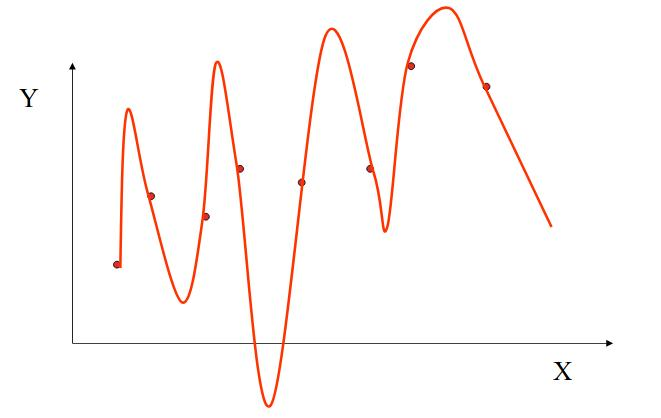
\includegraphics[scale = 0.3]{img/of.jpg}
  \caption{Esempio di modello in overfitting}
  \label{fig:over}
\end{figure}
Normalmente quindi si fa il testing su un testing set. Spesso è meglio avere un
modello meno preciso ma con complessità computazionale adeguata al dominio in
cui sto lavorando.
\begin{figure}
  \centering
  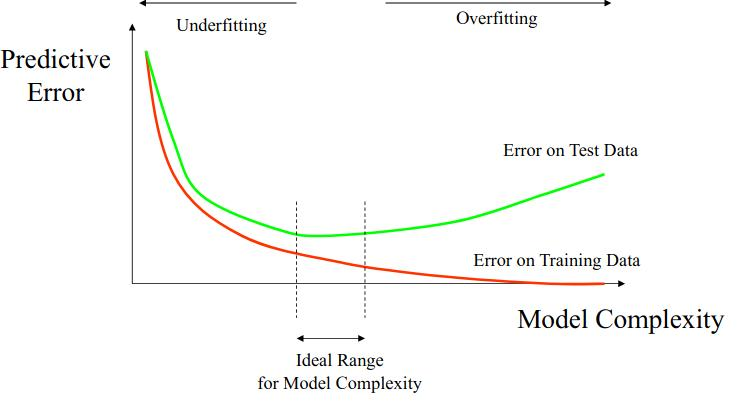
\includegraphics[scale = 0.5]{img/of2.jpg}
  \caption{Andamento di overfitting/underfitting sulla qualità del modello, con
    indicato il range ideale. Spesso sull'asse delle $x$ si ha il numero di
    iterazioni necessarie per capire quando terminarle per non andare in
    overfitting, come nel caso delle reti neurali}
  \label{fig:over2}
\end{figure}
Si hanno quindi varie misure di performance:
\begin{itemize}
  \item error rate e accuratezza
  \item true/false positive/negative
  \item precisione, recall, F-Measure
  \item curve ROC
  \item complessità temporale
\end{itemize}
Si hanno quindi:
\begin{itemize}
  \item successo, se le istanze sono predette correttamente
  \item errore, se le istanze non sono predette correttamente
\end{itemize}
Calcolando, per il primo punto:
\begin{itemize}
  \item l'error rate come percentuale di errori commessi sull'intera serie di
  istanze 
  \item accuratezza come proporzione d'istanze classificate correttamente
  sull'intero set d'istanze 
\end{itemize}
Passiamo al secondo punto.\\
Normalmente si munta a minimizzare falsi positivi/negativi anche se tutte e 4 le
entry della matrice di confusione andrebbero ottimizzate (con le entry che
possono avere costi 
diversi a seconda del dominio, si pensi alle diagnosi mediche dove i falsi
negativi sono più gravi dei falsi positivi).\\
In un problema multiclasse ho su righe e colonne le classi reali e le classi
predette, rispettivamente, non avendo più chiari i veri/falsi positivi/negativi,
che comunque possono essere ricavati per ogni classe.\\
\begin{definizione}
  Definiamo (in pratica per il caso binario):\\
  \textbf{accuratezza}:
  \[\frac{TP+TN}{TP+TN+FP+FN}\]
  (che nel caso multiclasse è la somma dei valori sulla diagonale principale
  diviso la somma del resto)\\
  \textbf{precisione}:
  \[\frac{TP}{TP+FP}\]
  \textbf{recall}:
  \[\frac{TP}{TP+FN}\]
  \textbf{F-measure}:
  \[\frac{2\cdot precisione\cdot recall}{precisione+ recall}\]
  \textbf{Queste sono le tradizionali misure globali.}
\end{definizione}
Si costruiscono quindi le matrici di confusione a seconda del caso binario o
multiclasse. Ma per il caso multiclasse posso calcolare solo la precisione di
una singola classe, come anche per recall e F-measure.\\
Spesso quindi si lavora a livello di classe.
\begin{definizione}
  Si hanno, data una label $l$ nell'insieme delle etichette $L$:\\
  \textbf{precisione}:
  \[P(l)=\frac{\# \text {of instances correctly predicted as } 1}{\#\text {of
        instances predicted as } 1}\]
  \textbf{recall}:
  \[R(l)=\frac{\# \text {of instances correctly predicted as } 1}{\#\text {of
        instances of class } 1}\] 
  \textbf{F-measure} (ovvero tramite media armonica):
  \[F(l)=\frac{2 \cdot P(l) \cdot R(l)}{P(l)+R(l)}\]
  Potrei avere un parametro $\beta$ per dare più importanza a una certa classe.
\end{definizione}
Si hanno modi per aggregare le misure di performance per scoprire comportamenti
particolari. 
\begin{definizione}
  Data un'etichetta $l$ ho due tecniche di aggregazione:\\
  \textbf{Macro-average} di una misura di performance $Perf$:
  \[\text {Perf}\,^{*}=\frac{1}{|L|} \sum_{i=1}^{|L|} \text {Perf}(l)\]
  dicendo che tutte le classi sono ugualmente importanti e hanno tutte lo stesso
  peso.\\
  \noindent
  \textbf{Micro-average} dove ho una media pesata:
  \[\text {Perf}\,^{*}=\sum_{l=1}^{|L|} \frac{|class(l)|}{\#\text{of istances}}
    \text {Perf}(l)\] 
  Dando quindi più peso alle classi più ``corpose'' e predominanti.
\end{definizione}
Parliamo ora di curve \textbf{Receiver Operating Characteristic (\textit{ROC})},
che rappresentano delle curve che dimostrano la 
capacità discriminativa di un modello al variare di una certa soglia. Si
confrontano veri/falsi positivi al variare di una certa soglia (che varia la
variabile sperimentale). Variare la
soglia permette di avere decisioni diverse e permette di costruire la curva
ROC. In problemi con tante classi, soprattutto se alcune sotto dimensionate, si
rischia di non riconoscerle queste classi ma abbassando la soglia si può aiutare
il modello a riconoscerle. \textbf{Si ha una curva ROC per ogni classe} (con una
soglia unica però). L'uso delle curve ROC è comodo per fare tuning su modelli
indotti da dati molto sbilanciati. Si confrontano i vari modelli a seconda delle
singole classi studiando l'impatto della soglia. 
\begin{figure}
  \centering
  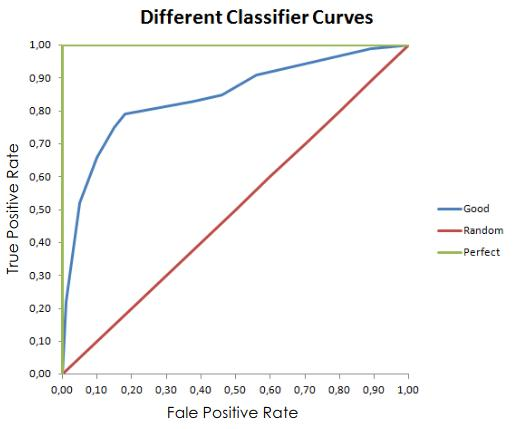
\includegraphics[scale = 0.5]{img/roc.jpg}
  \caption{Esempio di curva ROC per una certa classe. Se una curva, associata ad
    un certo metodo, domina tutte le altre allora quello è il metodo
    migliore. Se vale per ogni classe non si hanno più dubbi.}
  \label{fig:roc}
\end{figure}
Passiamo ora alla \textbf{learning curve}. Sono utili per studiare come evitare
l'overfitting, confrontando la cardinalità degli esempi con una miusra di
performance, come l'accuratezza. a un certo punto si arriva a un plateau e
quindi è inutile aumentare il numero di esempi (e la complessità computazionale)
se tanto non si hanno miglioramenti. Non solo, si aumenta anche la probabilità
di overfitting. 
\begin{figure}
  \centering
  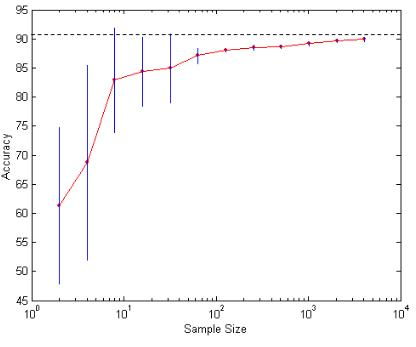
\includegraphics[scale = 0.5]{img/lc.jpg}
  \caption{Esempio di learning curve.}
  \label{fig:roc}
\end{figure}
Normalmente abbiamo lavorato con train e test (divisi circa per $\frac{2}{3}$ e
$\frac{1}{3}$, rispettivamente, per poi trainare il modello sul training e
testare i risultati sul test) ma questa è una visione parziale.  \\
In generale più è grande il test set e più accurata la stima
dell'errore. D'altro canto più è grande il training set e meglio sarà fatta la
classificazione, al più di overfitting. Il test set non deve essere usato per il
training e per il tuning ma si usa il validation set per il tuning, che quindi è
un set aggiuntivo usato per ottimizzare i parametri (soglia, parametro di
complessità della SVM etc$\ldots$) quando il dataset è abbastanza grande da
permetterlo. Il validation è solitamente il $10\%$ del training set.\\
Se il dataset è piccolo magari la divisione appena detta non è rappresentativa
ma si usano tecniche di \textbf{repeated holdout}, in cui si divide più volte
usando di volta i dati nei vari set. Si usa la \textbf{cross-validation} e la
\textbf{k-fold-cross-validation} dove si hanno due step:
\begin{enumerate}
  \item i dati vengono suddivisi in $k$ sottoinsieme di uguale dimensione 
  \item ogni sottoinsieme a sua volta viene utilizzato per il test e il resto
  per l'addestramento 
\end{enumerate}
pesso i sottoinsiemi vengono stratificati prima che venga eseguita la cross
validation e viene calcolata la media delle stime di errore per fornire una 
stima complessiva dell'errore.\\
Per costruire una matrice di confusione su una time-fold-convalidation
costruisco per ogni iterazione di folding la matrice di confusione dello
specifico test set e alla fine le si somma per ottenere la matrice finale.\\
Una variante è la \textbf{stratified ten-fold cross-validation} in quanto
esperimenti approfonditi hanno dimostrato che questa è la scelta migliore per
ottenere una stima accurata (usare 10 fold) e avendo che la distribuzione delle
istanze selezionate, rispetto alla classe da prevedere in ogni volta, è simile
alla distribuzione originale del set di dati (per lo stratified). La
stratificazione riduce la stima  
della varianza ma è ancora meglio ripetere tale stratificazione dieci volte.\\
Si hanno altre tecniche definite di \textbf{bootstrap} che utilizzano il
campionamento con rimpiazzo dal training set, avendo che la stessa istanza può
finire puiù volte nello stesso ``esperimento'' di time fold cross validation. Le
istanze del dataset originale che non compaiono nel nuoo training set vengono
usate come test. \textbf{Su slide 0.632 bootstrap, una tecnica empiricamente
  efficiente ma poco usata per la distorsione dei risultati a casua del suo
  pessimismo intrinseco}.\\
Una tecnica alternativa è \textbf{leave-one-out} che perfeziona il bootstrap. In
questa tecnica si ha una $k$ fold validation con $k$ pari al numero delle
istanze. Un'istanza sola viene lasciata per il test e tuutte le altre per il
training, cambiando ad ogni iterazione quella di testing fino ad esaurimento. È
computazionalmente pesante ($n$ fold per $n$ istanze) ma fa il miglior uso dei
dati. \\
Da un punto di vista metodologico vediamo ora come misurare la robustezza di un
modello, anche rispetto a un altro modello. Si misurano quindi gli
\textbf{intervalli di confidenza} per un certo livello di confidenza. Tra
modelli si confrontano quindi gli intervalli di confidenza, preferendo quello
con intervallo più stretto (per l'intervallo esempi con t-student). Oltre alle
misure già elencate precedentemente si 
usa anche l'entropia (\textbf{esempio su slide}).\\
Un secondo elemento per preferire un modello a un altro (dicendo che
``out-performa'' l'altro) è usare i \textbf{test di significatività}. Per farlo
si usa il \textbf{test della t-student} e se i due modelli stanno lavorando
sulla stessa configurazione di fold allora posso usare il \textbf{paired t-test}
confrontando direttamente le predizioni, non avendo variabilità sperimentale tra
i due risultati. \textbf{Sulle slide eventuali formule per il calcolo riprese
  dalle basi di statistica}.\\
Quindi:
\begin{itemize}
  \item si fissa il livello di significatività desiderato (normalmente $95\%$)
  \item si divide per due avendo un test a due cose
  \item si cerca il valore di $z$
  \item se $t\leq -z$ o $t\geq z$ la differenza è significativa
\end{itemize}
Potrebbe capitare che un t-test paired non sia effettuabile, anche solo se nel
mezzo del lancio dei modelli si ha un fattore di randomicità o avendo una $k$
diversa di fold convalidation.\\
In generale:
\begin{itemize}
  \item non basarsi solo sui numeri per le prestazioni
  \item guardare bene l'output del modello
  \item non trascurare la complessità del modello
\end{itemize}
\section{Modelli non supervisionati}
Si hanno diverse tecniche per studiare la bontà del clustering tra cui:
\begin{itemize}
  \item clustering tendency
  \item clustering quality
\end{itemize}
Per la \textbf{cluster tendency} ci dice che bisogna verificare se i dati hanno
una certa tendenza e che non siano punti distribuiti uniformemente nello
spazio. Per studiare la cosa all'aumentare delle dimensioni si usano:
\begin{itemize}
  \item \textbf{Hopkin statistic} che studia la probabilità che il dataset sia
  generato con distribuzione uniforme, campionando $N$ punti e calcolando la
  distanza da ogni punto rispetto al punto più vicino. Si genera quindi un
  dataset simulato, campionando da una distribuzione uniforme e infine si
  calcola con:
  \[H=\frac{\sum_{i=1}^{n} y_{i}}{\sum_{i=1}^{n} x_{i}+\sum_{i=1}^{n} y_{i}}\]
  $H$ (hopkin statistic) oltre $0.75$ indica clustering tendency al $90\%$ di
  livello di confidenza
  \item  \textbf{VAT algorithm} dove si calcola la matrice di dissimilarità e si
  mettono vicini gli elementi simili, creando una matrice a blocchi riducendo il
  problema ad due dimensioni, facilmente visualizzabile
\end{itemize}
In merito al \textbf{clustering quality} posso misurare misure interne
(silhouette, somma dei quadrati etc$\ldots$) ma anche esterne (precisione,
recall etc$\ldots$), qualora si abbia a che fare con anche le classi ottenute
dal cluster. Posso quindi fare t-test paired o unpaired a seconda della
situazione. 